\documentclass[xcolor=dvipsnames,10pt]{beamer}
\usepackage[english]{babel}
\usepackage[utf8]{inputenc}
\usepackage{pict2e}
\usepackage{colortbl}
\usepackage{graphicx}
\usepackage{pdfpages}
\usepackage{verbatim}
\usepackage{pgf}
%%%%%%%%%%%%%%%%%%%%
%%% nice math
\usepackage{amssymb}
\usepackage{amsmath}
\usepackage{latexsym}
\usepackage{amsthm}
\usepackage{slashed}
%%%%%%%%%%%%%%%%%%%%
%%% font type
%\usepackage{times}
\usepackage{bookman}
%\usepackage{palatino}
%\usepackage{newcent}
%\usepackage{avant}
\usefonttheme{serif}
\usepackage{atlasphysics}
%\usepackage{tikz}
\usepackage{subfigure}

\newcommand{\AC}{\ensuremath{\text{A}_{\text{C}}}}
\newcommand{\formatGenerator}[1]{\textsc{#1}}
\newcommand{\mcnlo}{\formatGenerator{mc@nlo}}
\newcommand{\wjets}{\ensuremath{W+\mathrm{jets}}}
\providecommand{\abs}[1]{\lvert#1\rvert}
\newcommand{\dy}{\ensuremath{\Delta{}\abs{y}}}
\newcommand{\deta}{\ensuremath{\Delta{}\abs{\eta}}}
\newcommand{\mtt}{\ensuremath{m_{\ttbar{}}}}
\newcommand{\Nupup}{\ensuremath{N(\uparrow\uparrow)}}
\newcommand{\Ndodo}{\ensuremath{N(\downarrow\downarrow)}}
\newcommand{\Nupdo}{\ensuremath{N(\uparrow\downarrow)}}
\newcommand{\Ndoup}{\ensuremath{N(\downarrow\uparrow)}}


%%% nice tables
\usepackage{booktabs}
\usepackage{multirow}
\usepackage{dcolumn}

\usepackage{fancybox}

%%% code pieces
\usepackage{listings}
\lstset{basicstyle=\tiny,language=c,emphstyle=\color{red},columns=fullflexible,
keepspaces=false, keywordstyle=\tiny\color{blue}, showstringspace=false} 
\newcommand\BackgroundPicture[1]{%
   \setbeamertemplate{background}{%
   \parbox[c][\paperheight]{\paperwidth}{%
       \vfill \hfill
\includegraphics[width=0.6\paperwidth,height=0.6\paperheight]{#1}
        \hfill \vfill
     }}}
\newcommand\FullBackgroundPicture[1]{%
   \setbeamertemplate{background}{%
   \parbox[c][\paperheight]{\paperwidth}{%
     \centering\vspace{2cm} \vfill 
\includegraphics[width=0.8\paperwidth,height=0.7\paperheight]{#1}
\vfill 
     }}}

%\setbeamertemplate{headline}

%%% to allow small margin
\newenvironment{changemargin}[2]{%
  \begin{list}{}{%
    \setlength{\topsep}{0pt}%
    \setlength{\leftmargin}{#1}%
    \setlength{\rightmargin}{#2}%
    \setlength{\listparindent}{\parindent}%
    \setlength{\itemindent}{\parindent}%
    \setlength{\parsep}{\parskip}%
  }%
  \item[]}{\end{list}} 

%\usetheme{Luebeck}
%\usecolortheme{seagull}
%\usecolortheme[named=BrickRed]{structure}


\usetheme[headheight=.13\textheight,footheight=.035\textheight]{boxes}
\definecolor{light-gray}{gray}{0.9}
%\definecolor{myfading}{fg=white,bg=light-gray}
\definecolor{structure2}{rgb}{1,1,1}

\mode<presentation>
%\usecolortheme[named=Black]{structure}
%\usecolortheme[named=Plum]{structure}
%\usecolortheme[named=Violet]{structure}
%\usecolortheme[named=BurntOrange]{structure}
%\usecolortheme[named=RedViolet]{structure}
\usecolortheme[named=Sepia]{structure}
\setbeamercolor{normal text}{fg=black!70!light-gray,bg=white}
\setbeamercolor{alerted text}{fg=BrickRed,bg=light-gray}
\setbeamercolor{boxcolor}{fg=black!70!light-gray,bg=structure!30!white}
\setbeamercolor{whiteboxcolor}{fg=black!70!light-gray,bg=white}

\definecolor{links}{named}{Plum}

\usepackage{hyperref}
\hypersetup{colorlinks=true,linkcolor=,urlcolor=links}

\setbeamercolor{head/foot boxes}{fg=structure!90!white,bg=structure!30!white}
\setbeamercolor{head/foot boxes bis}{fg=structure!60!white,bg=structure!90!white}

\setbeamercolor{head/foot text}{fg=structure!40!black,bg=structure!30!white}

%\addheadboxtemplate{\usebeamercolor[bg]{head/foot boxes}}{\usebeamercolor[fg]{head/foot text}\logo{\includegraphics[height=1.2cm]{pics/atlasifae2}}\raisebox{-1.8ex}{\insertlogo}\hfill\insertshorttitle \hskip0.3cm}
\addheadboxtemplate{\usebeamercolor[bg]{head/foot boxes}}{\usebeamercolor[fg]{head/foot text}\insertsubsectionhead \hskip0.3cm}
\addheadboxtemplate{\usebeamercolor[fg]{head/foot boxes}}{\usebeamercolor[bg]{head/foot text}\scriptsize\hskip0.3cm\insertsectionhead}

\addfootboxtemplate{\usebeamercolor[fg]{head/foot boxes}}{\usebeamercolor[bg]{head/foot text}\hskip0.3cm\insertshortauthor\\\insertshortinstitute \hfill}
\addfootboxtemplate{\usebeamercolor[fg]{head/foot boxes bis}}{\usebeamercolor[fg]{head/foot text}\hfill\insertdate\hfill}

\def\insertpresentationendframe{\inserttotalframenumber}
\makeatletter
\g@addto@macro{\appendix}{\immediate\write\@auxout{\string\@writefile{nav}{\noexpand\headcommand{\noexpand\def\noexpand\insertpresentationendframe{\the\c@framenumber}}}}}
\makeatother

\addfootboxtemplate{\usebeamercolor[bg]{head/foot boxes}}{\usebeamercolor[fg]{head/foot text}\hfill\insertframenumber/\insertpresentationendframe\hskip0.3cm}
%\addfootboxtemplate{\usebeamercolor[bg]{head/foot boxes}}{\usebeamercolor[fg]{head/foot text}\hfill\insertframenumber/\insertpresentationendpage\hskip0.3cm}

%\setbeamertemplate{footline}{%
%  \begin{beamercolorbox}{section in head/foot}
%\begin{center}
%\begin{tabular}{lcr}
%\hskip45pt \textit{Barcelona plans for u4u4 searches in lepton+jets} \phantom{a/aa} & 2011, December 21st \phantom{a/aa} \insertframenumber / %\insertpresentationendpage
%\\
%\end{tabular}
%\end{center}  \end{beamercolorbox}
%}


%\usesectionheadtemplate
%{\color{white}\tiny\textbf{\insertsectionhead}}
%{\color{structureshaded}\tiny\textbf{\insertsectionhead}}


%\useoutertheme{sidebar}
%\setbeamertemplate{sidebar canvas left}[vertical shading][top=White,bottom=Gray]
%\setbeamertemplate{sidebar canvas left}[vertical shading][top=White,bottom=CadetBlue]
%\setbeamertemplate{sidebar canvas left}[vertical shading][top=White,bottom=YellowGreen]
%\setbeamertemplate{sidebar canvas left}[vertical shading][top=White,bottom=light-gray]

\setbeamertemplate{navigation symbols}{}
\setbeamersize{text margin left=.2cm,text margin right=.2cm} 






\AtBeginSection[]
{
  \begin{frame}\centering
    \frametitle{Outline}
    \tableofcontents[currentsection]
  \end{frame}
}



\title[Probing new physics at the LHC: \\ searches for heavy top-like quarks \\ with the ATLAS experiment]{{\bfseries Probing new physics at the LHC: \\ searches for heavy top-like quarks \\ with the ATLAS experiment}}
\author[A Succurro]{Antonella Succurro\\ \vspace{\baselineskip}\textit{\small PhD candidate in Physics}\vspace{-0.7cm}}
\institute[\, \emph{IFAE, UAB}]{
\begin{tabular}{p{0.25\textwidth} p{0.25\textwidth} p{0.25\textwidth}}
  \vspace{0.7cm} 
\includegraphics[width=2.5cm]{../smallstuff/ifae_logo.pdf}\hspace{0.2cm}&
  \vspace{0.5cm} \includegraphics[width=2.8cm]{../smallstuff/uab_logo.pdf}&
  \vspace{0.cm} \hspace{0.5cm} \includegraphics[width=1.5cm]{pics/atlas_logo}\\
\end{tabular}
}
\date{Bellaterra, 28th of February, 2014}

\definecolor{LightCyan}{rgb}{0.88,1,1}
\def\cccolor{\usebeamercolor[fg]{head/foot boxes}}

\begin{document}


\frame{

\vspace{-.8cm}

\maketitle\centering

\vspace{-.8cm}
}



\begin{frame}\frametitle{Four questions, one dissertation}

%{\large\bfseries
%\usebeamercolor[fg]{head/foot boxes}
%\dots one thesis\dots
%}

%\myskip

%\pause
\centering
  \begin{minipage}{.5\textwidth}\centering

%\myskip

\begin{itemize}[<+->]
\item {\cccolor \LARGE Why?} {\scriptsize bother with ``new physics''}
\item {\cccolor \LARGE Where?} {\scriptsize is all happening}
\item {\cccolor \LARGE What?} {\scriptsize are we looking at}
\item {\cccolor \huge How?} {\scriptsize}
\end{itemize}

\end{minipage}

%\pause
%\flushright
%{\large\bfseries
%\usebeamercolor[fg]{head/foot boxes}
%\dots no solution! (yet)
%}


\end{frame}

%\begin{frame}\frametitle{Content}
%\end{frame}
%\begin{frame}\frametitle{Outline}
%\centering
%\tableofcontents[part=1,pausesections]
%\tableofcontents
%\end{frame}

%----------------------------------
%\section{Introduction}
%----------------------------------
%\begin{frame}\frametitle{Standard Model as an effective theory}
%\scriptsize\centering
%\end{frame}


%----------------------------------
\section{Theoretical framework}
%----------------------------------

\begin{frame}\frametitle{Standard Model as an effective theory}
\scriptsize\centering

\myskip
\end{frame}



%----------------------------------
\section{The ATLAS experiment at the LHC}
%----------------------------------

\FullBackgroundPicture{../detector/figures/ring}

\begin{frame}\frametitle{The LHC complex}
\footnotesize\centering
\begin{minipage}{.9\textwidth}
%\end{minipage}\begin{minipage}{.6\textwidth}\centering\pause

\pause
\begin{beamercolorbox}[wd=.99\textwidth,rounded=true,shadow=true]{whiteboxcolor}\centering\scriptsize
	\begin{tabular}{lllll}\toprule
        Parameter                       & designed      &       2010 &  2011     &   2012\\ \midrule
        Beam energy (\tev/c)            & 7             & 3.5        & 3.5       & 4    \\
        Beta function $\beta*$ (m)      & 0.55          & 2.0/3.5    & 1.5/1.0   & 0.6  \\
        Max. No. bunches/beam           & 2808          & 368        & 1380      &1380  \\
        Max. No. protons/bunch          & 1.15$\times10^{11}$ & 1.2$\times10^{11}$ & 1.45$\times10^{11}$ & 1.7$\times10^{11}$ \\
        Bunch spacing (ns)              & 25            & 150       & 75/50        & 50 \\
        Peak luminosity (\cmm2\sm1)     & 1$\times10^{34}$& 2.1$\times10^{32}$& 3.7$\times10^{33}$& 7.7$\times10^{33}$\\
        Emittance $\varepsilon_{n}$ ($\mu$rad)&3.75     &   2.0      & 2.4      & 2.5   \\
        Max. $<\mu>$                    & 19            & 4             & 17         & 37       \\
	\bottomrule\end{tabular}

\end{beamercolorbox}

\end{minipage}

\myskip

\end{frame}


\FullBackgroundPicture{../detector/figures/atlas}

\begin{frame}\frametitle{The ATLAS Detector}
\footnotesize\centering

\begin{minipage}{.7\textwidth}\centering

\only<2>{
\hspace{2cm}\begin{beamercolorbox}[wd=.9\textwidth,rounded=true,shadow=true]{whiteboxcolor}\centering
{\bfseries In 2012 20.3~\ifb\  collected at $\sqrt{s}=8~$TeV!}
\vspace{.3cm}

\includegraphics[width=.8\textwidth]{pics/intlumivstime2012DQ}

\vspace{\baselineskip}
%Reached peak luminosity of $3.65\times 10^{33}~$cm$^{-2}$s$^{-1}$\\
\end{beamercolorbox}
}

\end{minipage}

%Will present results obtained with \alert{14.3\ifb}\ of 2012 data

\end{frame}

\BackgroundPicture{pics/emptyIMG}

%----------------------------------
\section{Monte Carlo simulation}
%----------------------------------

\begin{frame}\frametitle{Modelling of hadron collisions}
\small\centering

want to do physics at hadron colliders?

need a good understanding of incoming hadrons

\myskip
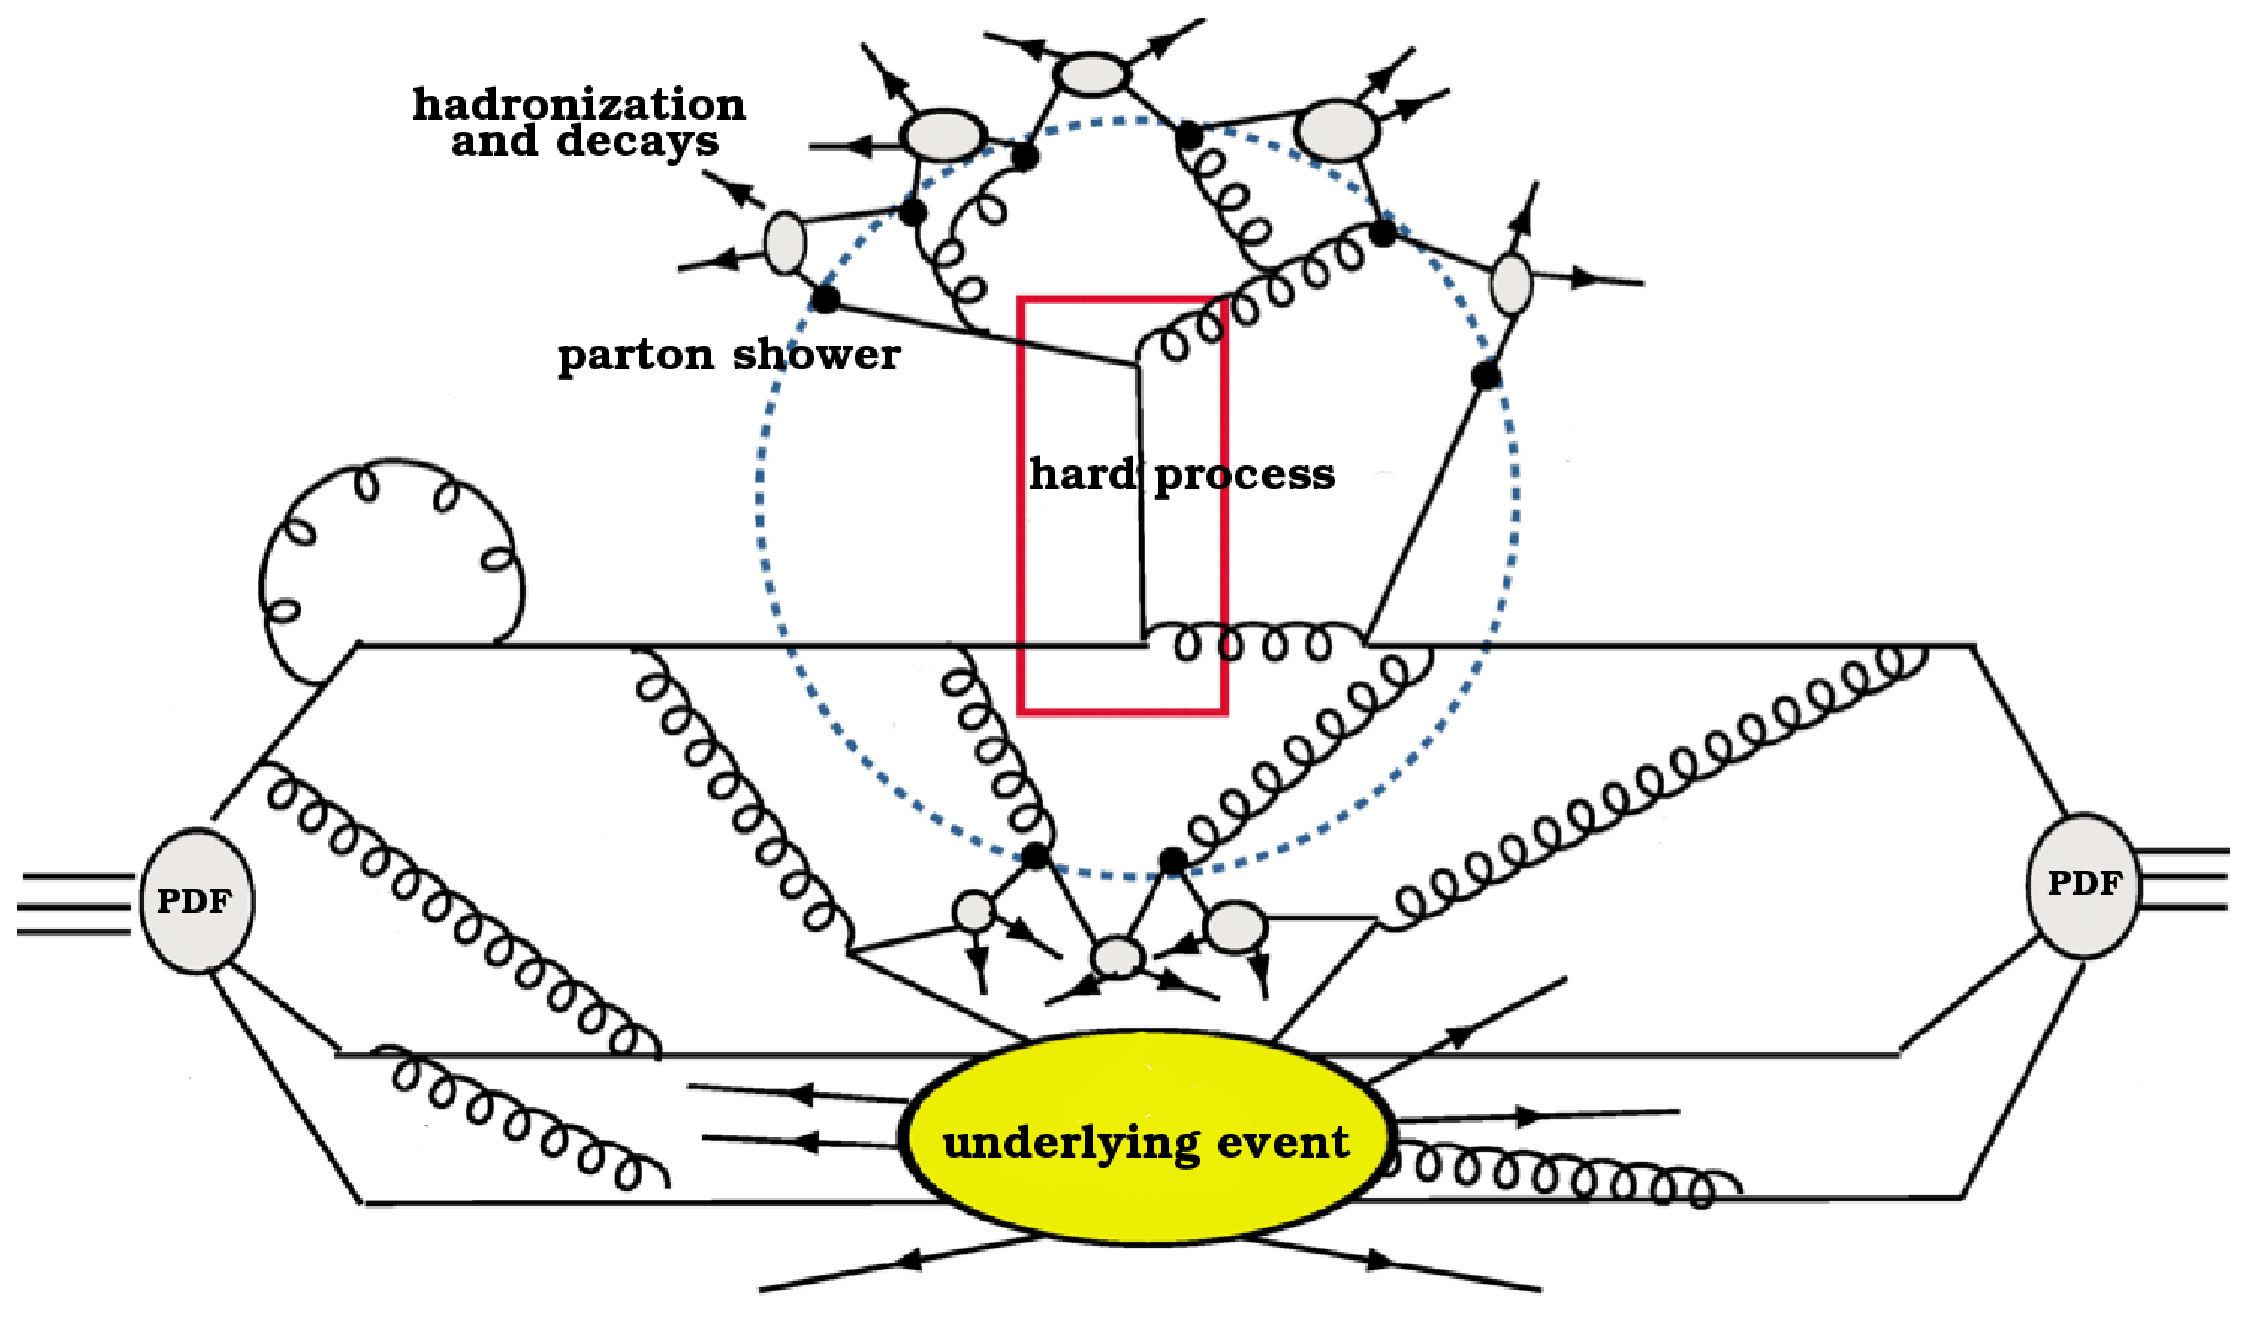
\includegraphics[width=.7\textwidth]{../montecarlo/figures/my_collision}

\end{frame}

%%%% EVENT1
\FullBackgroundPicture{../montecarlo/figures/event1}
\begin{frame}\frametitle{Modelling of hadron collisions}

\begin{flushright}\tiny Drawings from~\cite{Gieseke}\end{flushright}

\centering\myskip
%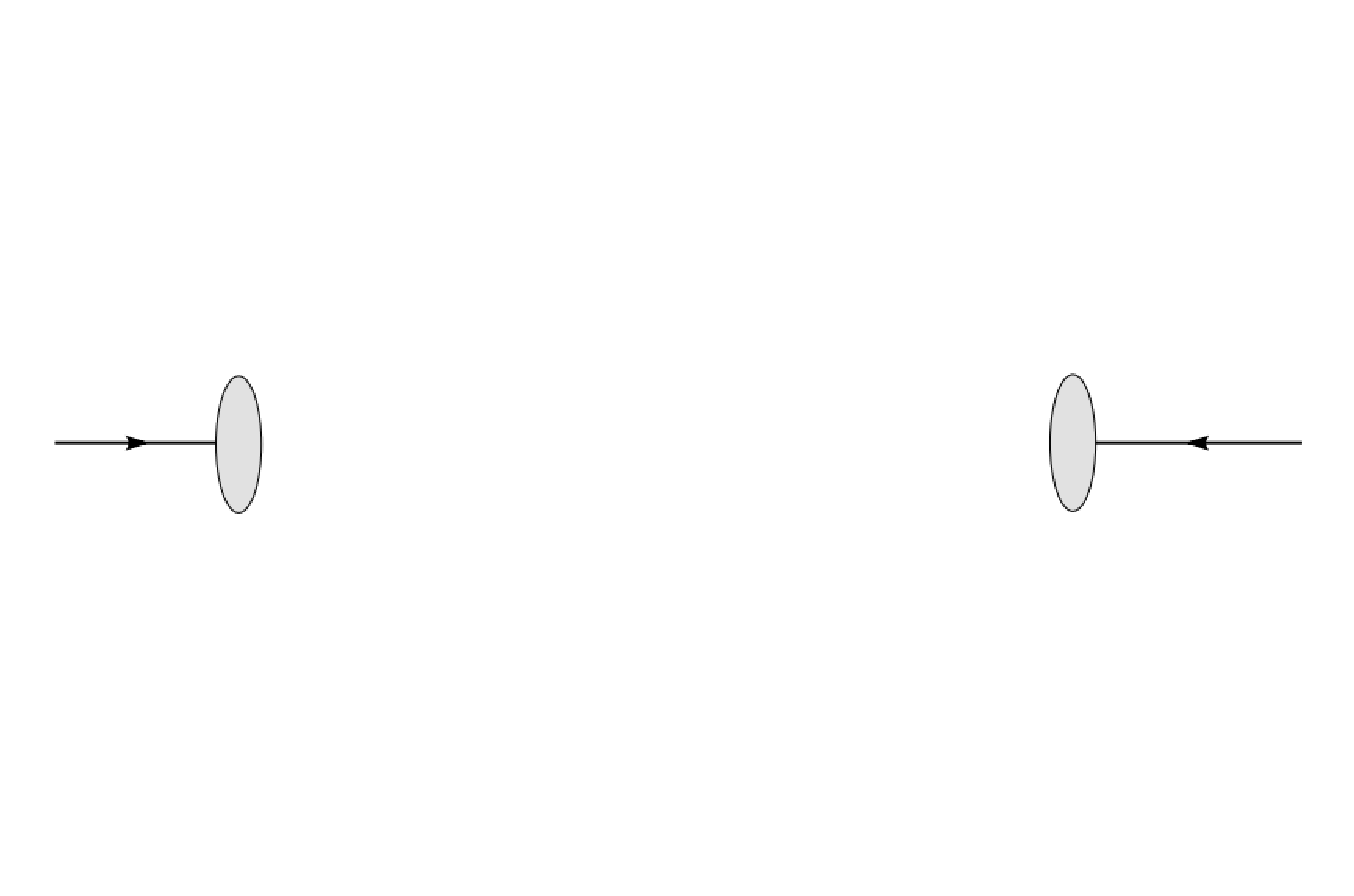
\includegraphics[height=0.8\textheight]{../montecarlo/figures/event1}

$E(p_1)=4\tev$ \hspace{.3\paperwidth} $E(p_2)=4\tev$

\vspace{.3\paperheight}

Quarks are distributed according to PDFs inside the proton\\
{\LARGE $\Downarrow$}\\
intial energy unknown

\end{frame}


%%%% EVENT1
\FullBackgroundPicture{../montecarlo/figures/event2}
\begin{frame}\frametitle{Hard scattering of two partons}
%\begin{flushright}\tiny Drawings from~\cite{Gieseke}\end{flushright}
\centering\myskip
%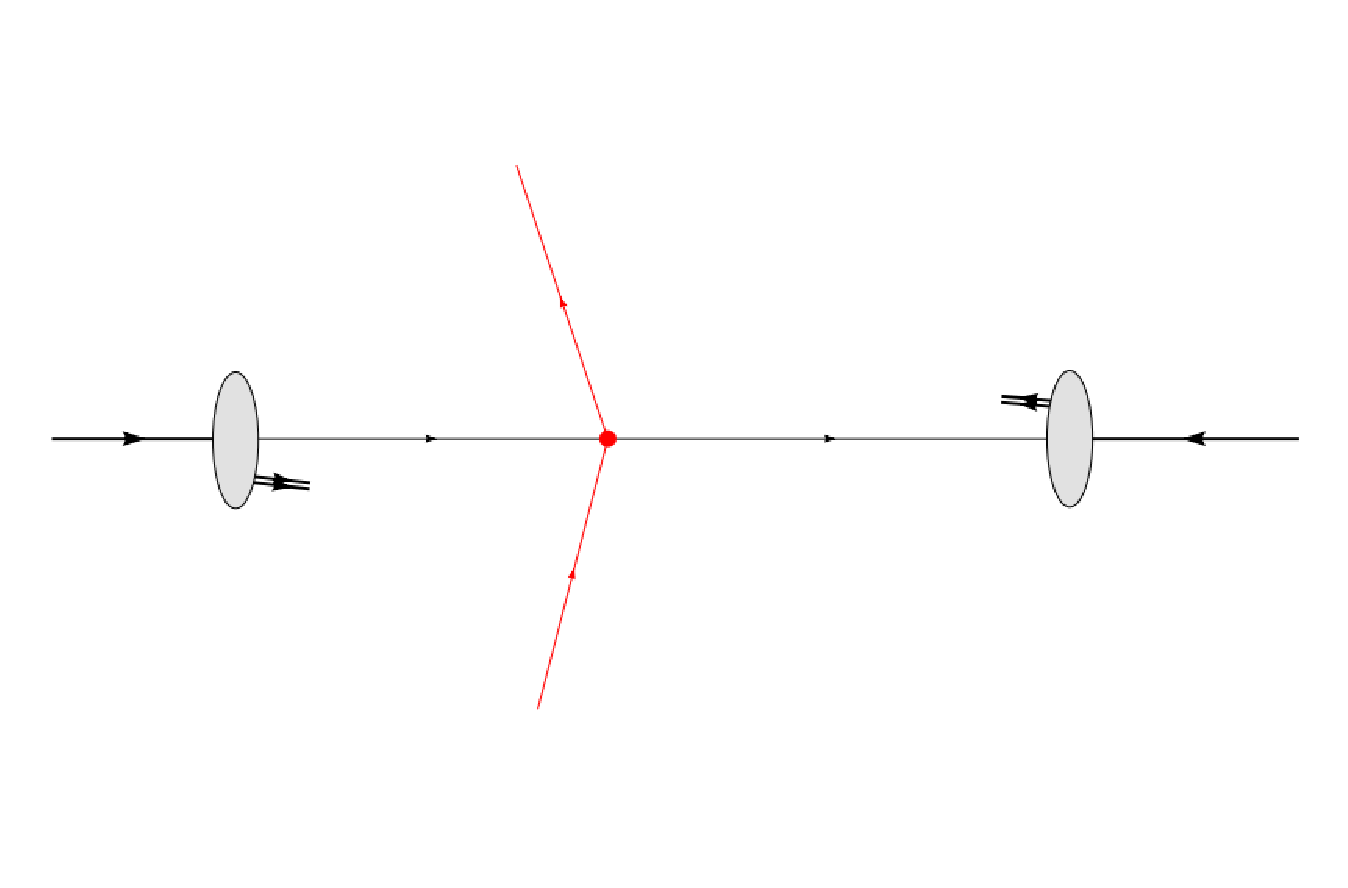
\includegraphics[height=0.8\textheight]{../montecarlo/figures/event2}


\vspace{.4\paperheight}

{\cccolor asymptotic freedom}: high energy $\longleftrightarrow$ low \alphas\\
{\LARGE $\Downarrow$}\\
(fixed order) pQCD

\end{frame}

%%%% EVENT1
\FullBackgroundPicture{../montecarlo/figures/event4}
\begin{frame}\frametitle{Parton showering}
\centering\myskip
%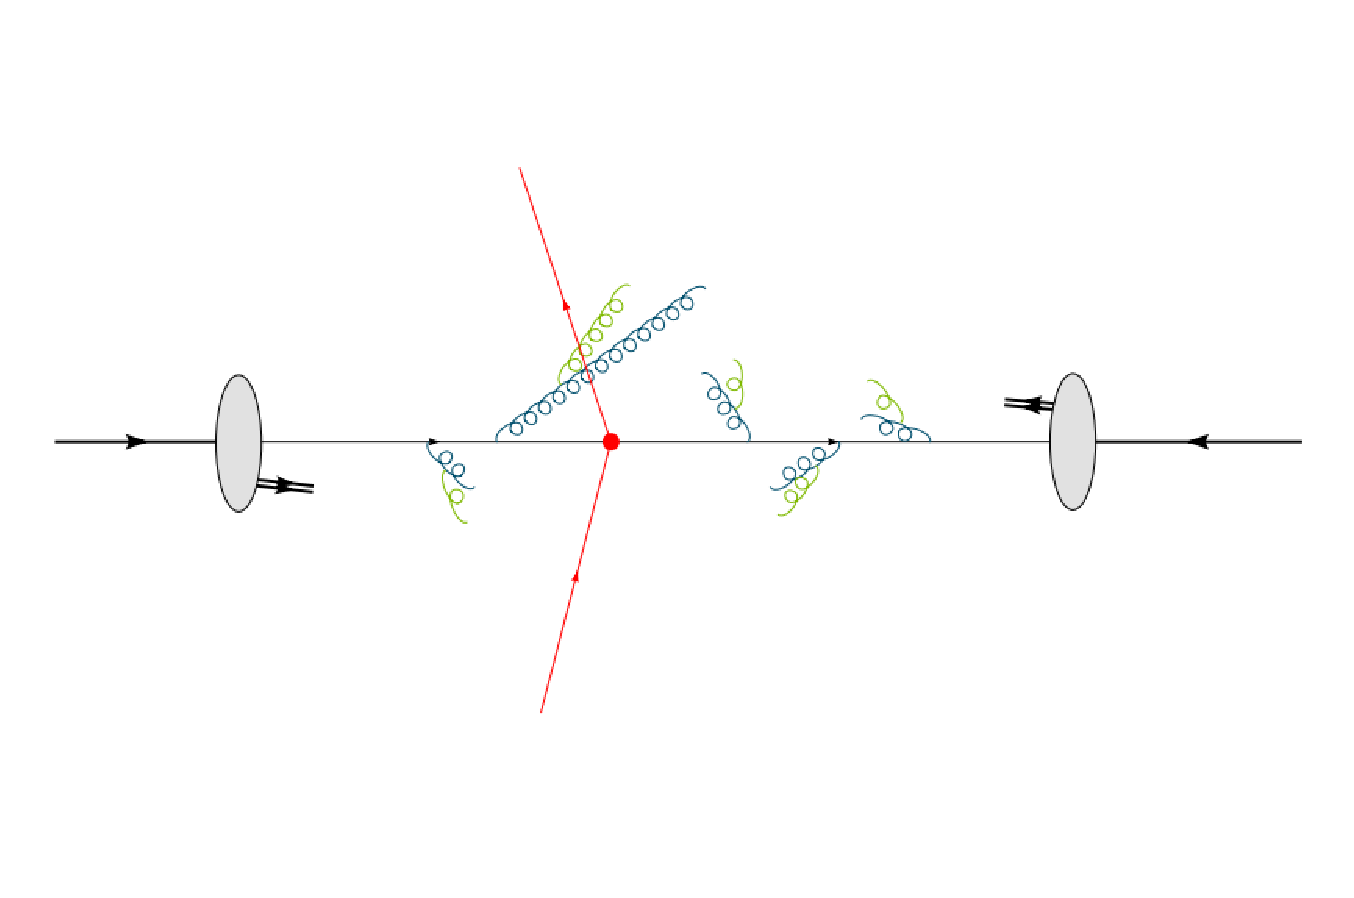
\includegraphics[height=0.8\textheight]{../montecarlo/figures/event4}

\vspace{.4\paperheight}

%real radiative corrections to any inclusive quantity

QCD emission: $q\to gq$, $g\to gg$, $g\to q\bar{q}$\\
{\LARGE $\Downarrow$}\\
higher-order corrections 

%\begin{flushright}\tiny Drawings from~\cite{Gieseke}\end{flushright}

\end{frame}

%%%% EVENT1
\FullBackgroundPicture{../montecarlo/figures/event6}
\begin{frame}\frametitle{Hadronization}
\centering\myskip
%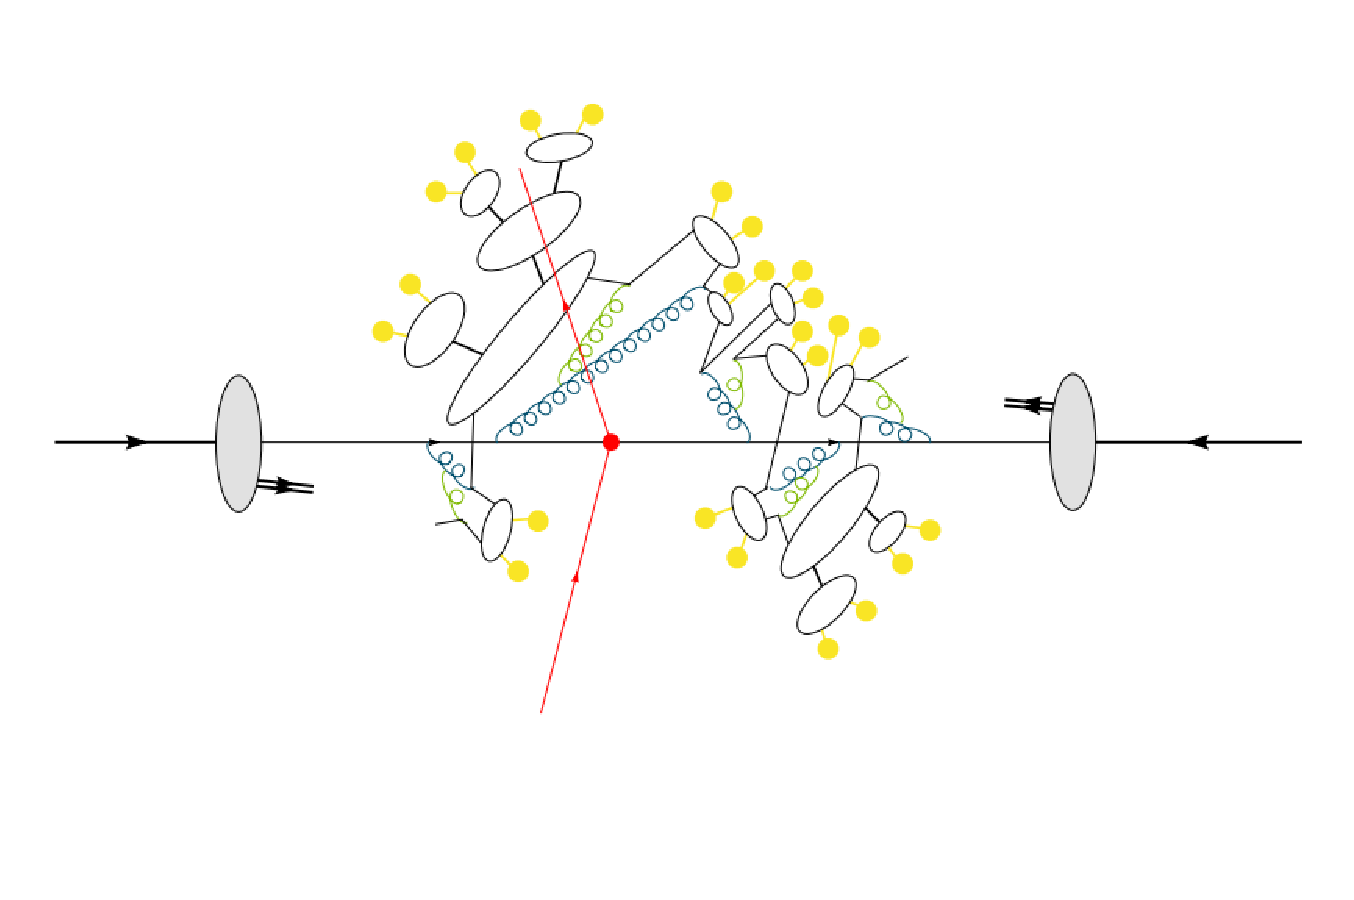
\includegraphics[height=0.8\textheight]{../montecarlo/figures/event5}


\vspace{.4\paperheight}

%\begin{flushright}\tiny Drawings from~\cite{Gieseke}\end{flushright}

\end{frame}


%%%% EVENT1
\FullBackgroundPicture{../montecarlo/figures/event7}
\begin{frame}\frametitle{Underlying event simulation}
\centering\myskip
%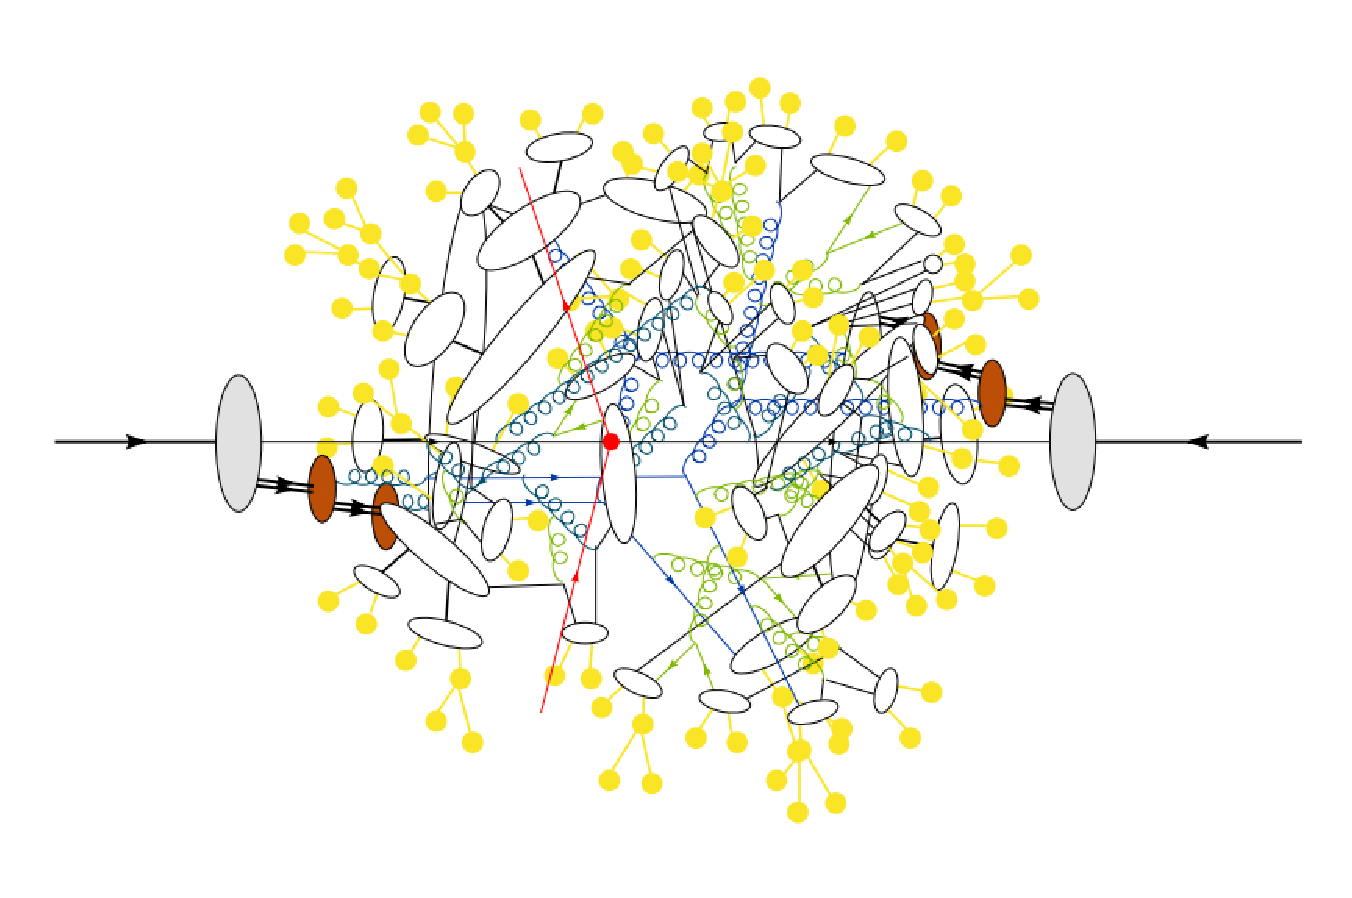
\includegraphics[height=0.8\textheight]{../montecarlo/figures/event7}


\vspace{.4\paperheight}

%\begin{flushright}\tiny Drawings from~\cite{Gieseke}\end{flushright}

\end{frame}


\BackgroundPicture{pics/emptyIMG}
\begin{frame}\frametitle{Pile-up}
\centering\myskip

\begin{minipage}{.35\textwidth}\centering
\footnotesize

But \sout{problems} collisions\\
never come alone\dots

\begin{itemize}
\item {\cccolor in-time} and {\cccolor out-of-time} pile-up events
\end{itemize}

\includegraphics[width=1.\textwidth]{pics/mu_2011_2012-dec.pdf}

\end{minipage}\begin{minipage}{.65\textwidth}\centering

\vskip-5ex
\footnotesize
2012 $Z\to\mu\mu$ event with high pile-up (25 vertices)

\includegraphics[height=0.9\textheight,width=1.\textwidth]{pics/2012_highPileup.png}

\tiny
from \url{https://twiki.cern.ch/twiki/bin/view/AtlasPublic/EventDisplayStandAlone}
\end{minipage}

\end{frame}

\BackgroundPicture{pics/emptyIMG}

%----------------------------------
\section{Event reconstruction}
%----------------------------------

\begin{frame}\frametitle{Physics objects puzzle}
\centering\myskip

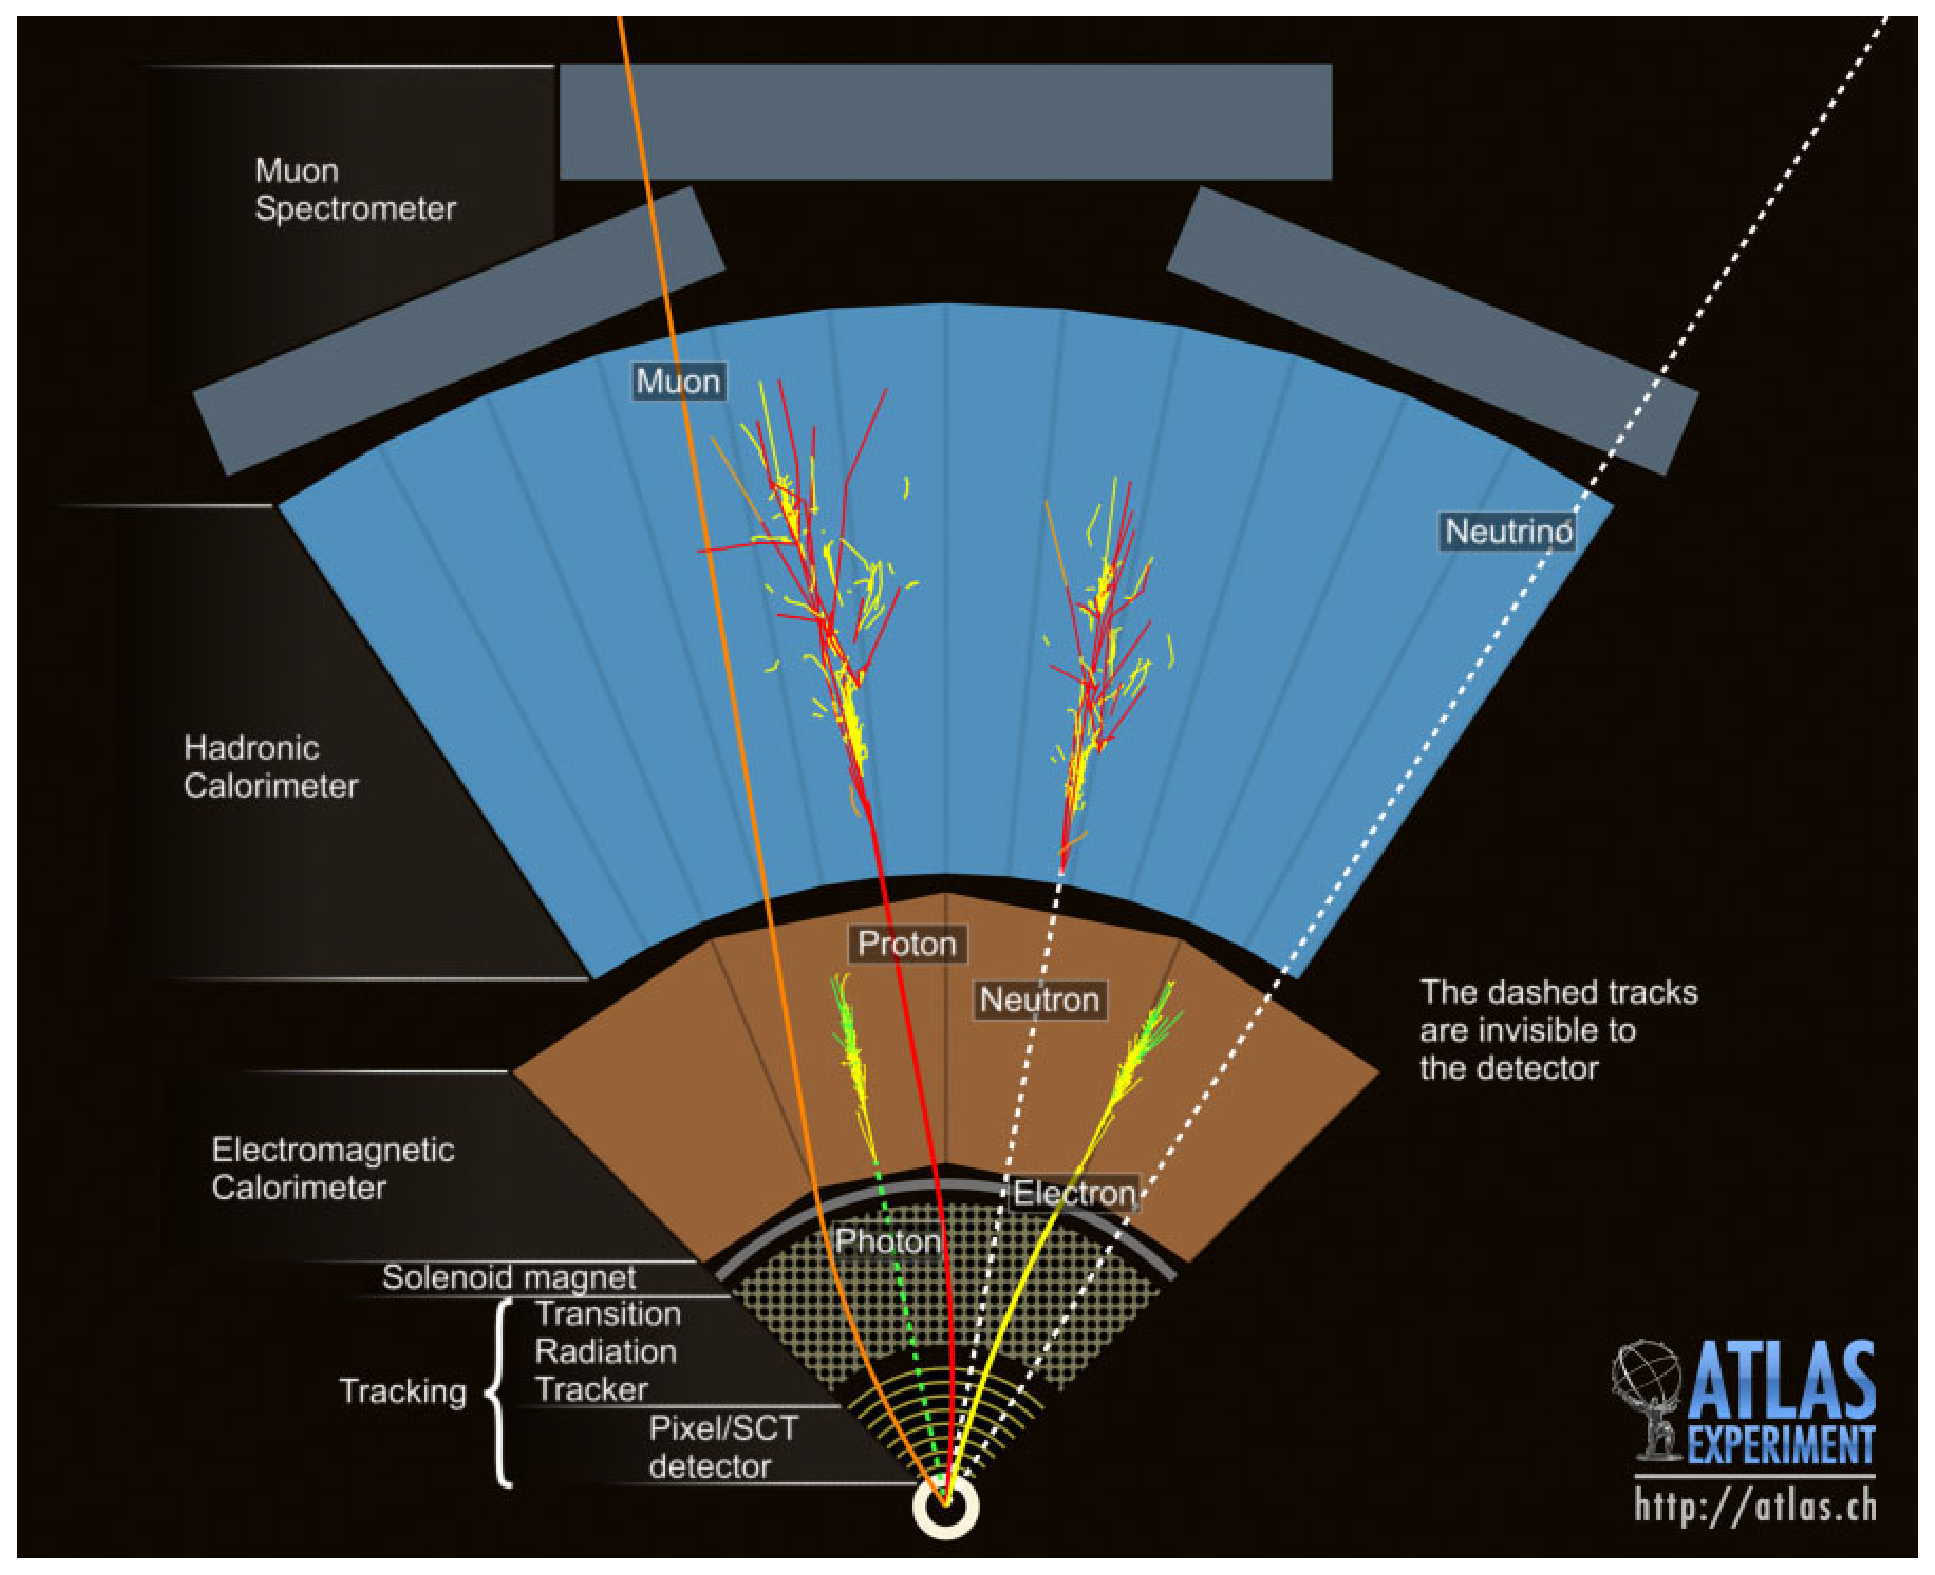
\includegraphics[height=0.85\textheight, width=1.\textwidth]{../detector/figures/detection}

\end{frame}



\begin{frame}\frametitle{One lepton}
\footnotesize\centering

\begin{minipage}{.5\textwidth}\centering
\includegraphics[width=.9\textwidth,height=0.3\textheight]{pics/Zee}

\begin{itemize}
\item $|\eta|<2.47$ ID track $\leftrightarrow$ EM deposit
\item $E_{\rm calo}$ consistent with $p_{\rm T, ID}$
\item calibrated with $Z\to ee$ events
\end{itemize}
{\cccolor \bfseries +}\\
\begin{itemize}
\item excluded $1.37< |\eta|< 1.52$
%\item $\et = E_{\rm cluster}/\cosh\eta_{\rm track} > 25\gev$, $|z_0|<2~$mm.
\item $\et > 25\gev$, $|z_0|<2~$mm
\item isolation cuts {\scriptsize\texttt{EtCone20}, \texttt{PtCone30}}
\item electron-jet overlap removal
\item {\scriptsize\texttt{EF\_e24vhi\_medium1} $||$ \texttt{EF\_e60\_medium1}}
\end{itemize}


\end{minipage}\begin{minipage}{.5\textwidth}\centering


\begin{itemize}
\item \texttt{Muid}: MS track $\leftrightarrow$ ID track ($|\eta|<2.47$)
\item $p_{\rm T,MS}$ corrected for mip loss
\item $p_{\rm T}$ weighted average MS $\leftrightarrow$ ID
\item calibrated with $Z\to \mu\mu$ events
\end{itemize}
{\cccolor \bfseries +}\\
\begin{itemize}
\item $\pt > 25\gev$, $|z_0|<2~$mm
\item isolation cut \texttt{PtCone20}
\item mini-isolation cut
\item \texttt{EF\_mu24i\_tight} $||$ \texttt{EF\_mu36\_tight}
\end{itemize}

\includegraphics[width=.78\textwidth,height=0.3\textheight]{pics/Zmumu}

\end{minipage}


\end{frame}



\begin{frame}\frametitle{Many jets}
\centering\footnotesize

\begin{minipage}{.5\textwidth}\centering

\includegraphics[width=.78\textwidth]{pics/Sketch_PartonParticleCaloJet.png}\\
%\resizebox{1.\textwidth}{!}{from \url{http://cms.web.cern.ch/news/jets-cms-and-determination-their-energy-scale}}

\begin{itemize}
\item Combine calorimeter clusters using anti-$k_t$ algorithm with $R=0.4$
\end{itemize}
$d_{ij}=min(\dfrac{1}{k_{t_i}^{2}},\dfrac{1}{k_{t_j}^{2}})\frac{\Delta R_{ij}^{2}}{R^{2}}$
\begin{itemize}
\item LC clusters energy
\item Pile-up and JES correction
\end{itemize}
{\cccolor \bfseries +}\\
\begin{itemize}
\item $\pt>25\gev$, $|\eta|<2.5$
\item JVF$>0.5$
\item jet-electron overlap removal
\end{itemize}


\end{minipage}\begin{minipage}{.5\textwidth}\centering
\includegraphics[width=.78\textwidth]{pics/antikt}\\
\includegraphics[width=.9\textwidth]{pics/corr_jet_lcw}

\end{minipage}


\end{frame}



\begin{frame}\frametitle{\btag ging}
\centering\footnotesize

\begin{minipage}{.3\textwidth}\centering

$b$ quark $\Rightarrow$ $B$ hadron ($\lambda\sim 10^{-12}$~s)\\
{\large$\Downarrow$}\\
travels about 3~mm\\ before decaying

\includegraphics[width=.8\textwidth]{../objectsreconstruction/figures/Picture-b-tagging-2.png}

\end{minipage}\begin{minipage}{.7\textwidth}\centering

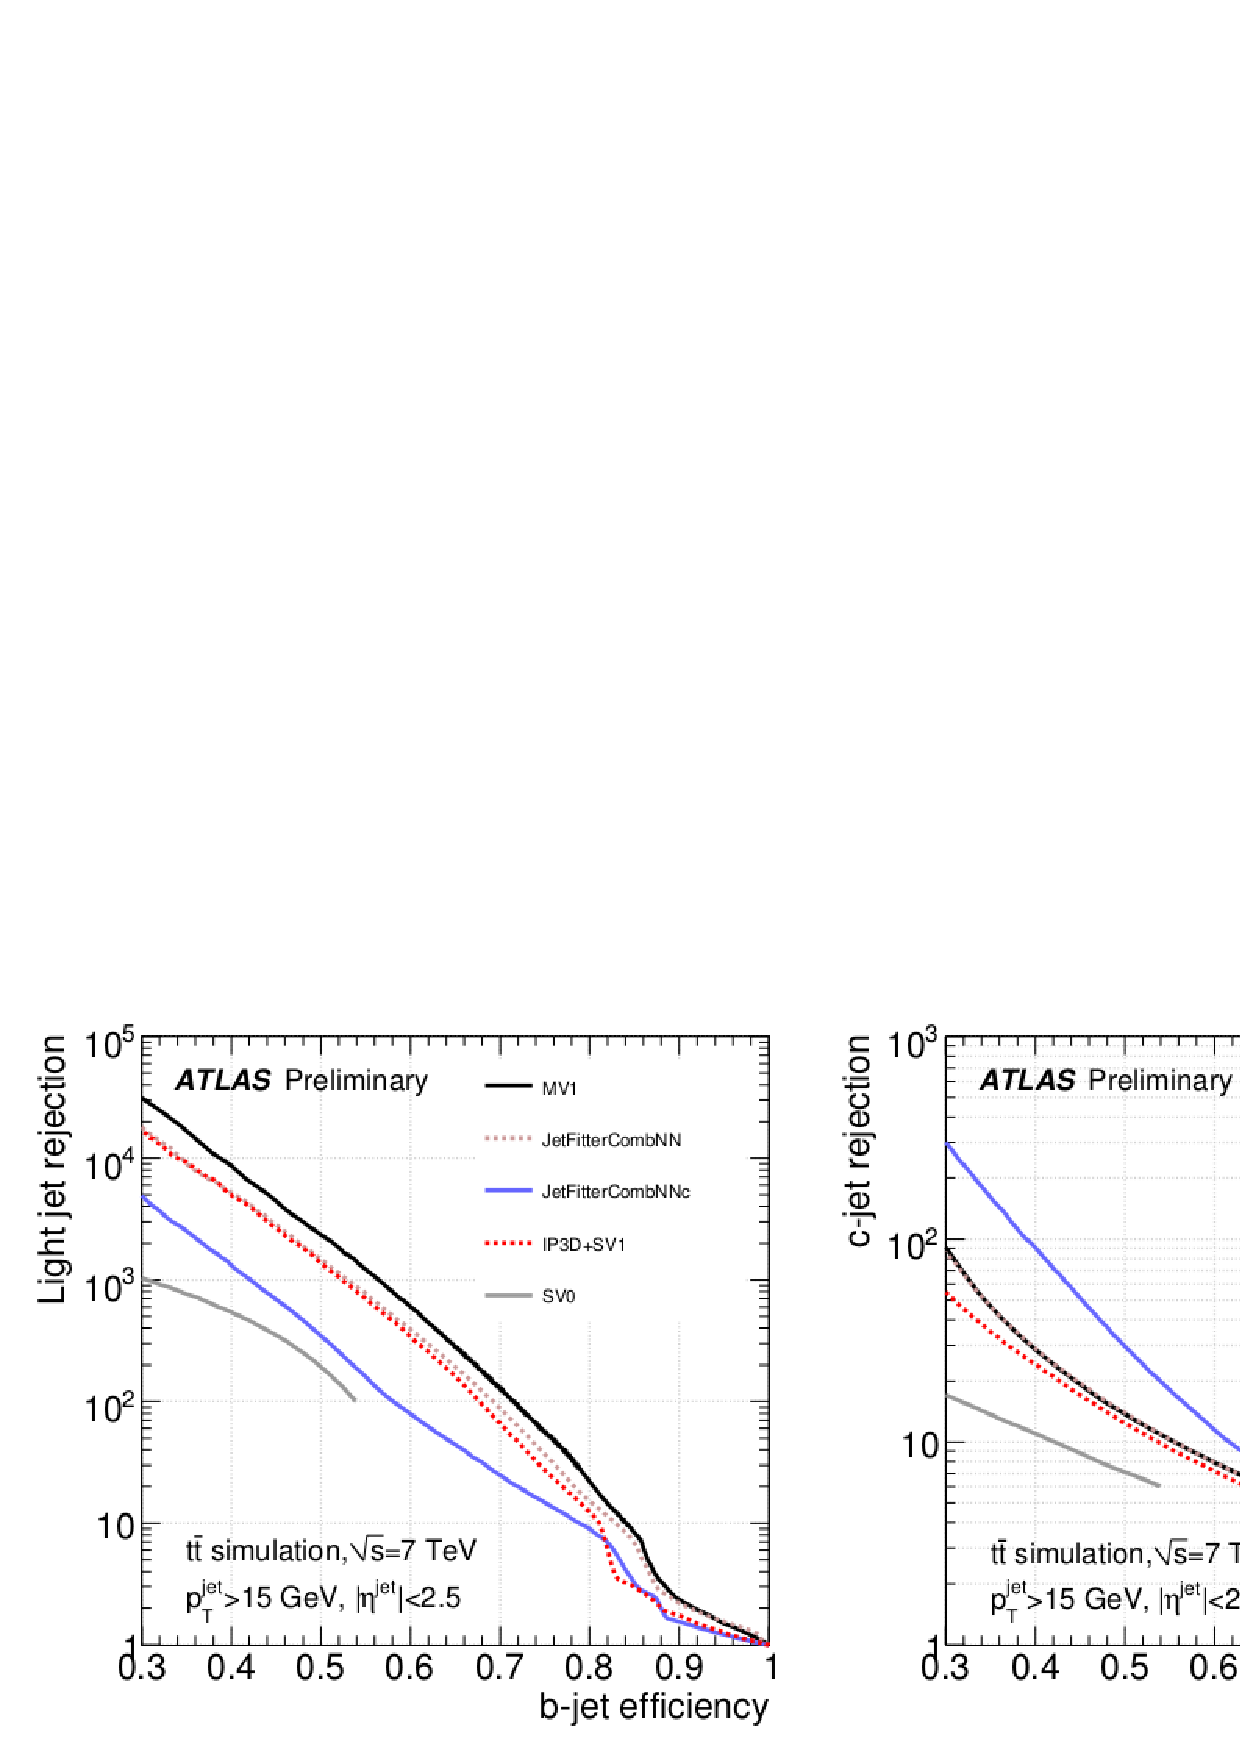
\includegraphics[width=1.\textwidth]{../objectsreconstruction/figures/btageffs.png}

\end{minipage}

\myskip

\begin{minipage}{.4\textwidth}\centering


various algorithms exploit ID track info to identify \bjet s

\begin{itemize}
\item \texttt{\cccolor MV1} algorithm @ 70\% efficiency, $\sim 130$ rejection
\end{itemize}

\end{minipage}\begin{minipage}{.6\textwidth}\centering

Events are selected through \\a cut on the \btag-weight computed\\
{\large$\Downarrow$}\\
with 70\% efficiency, high multiplicities will suffer

\begin{itemize}
\item {\cccolor TagRateFunction} method
\end{itemize}


\end{minipage}


\end{frame}



\begin{frame}\frametitle{Missing transverse energy}
\centering\myskip

\begin{minipage}{.5\textwidth}\centering

\includegraphics[width=.9\textwidth]{pics/real_et}\\
{\tiny from \url{http://tomwhyntie.wordpress.com/research/}}

\end{minipage}\begin{minipage}{.5\textwidth}\centering
\end{minipage}
$$\begin{array}{lcl}
%E^{\rm miss}_{x,y} & = & E^{\rm RefEle}_{x,y} + E^{\rm RefGamma}_{x,y} + E^{\rm RefJet}_{x,y} + E^{\rm RefMuon}_{x,y} + E^{\rm SoftJet}_{x,y} + E^{\rm CellOut}_{x,y}\\
E^{\rm miss}_{T} & = & \big|-\sum\vec{p}_T \big| = \sqrt{(E^{\rm miss}_{x})^2 + (E^{\rm miss}_{y})^2} ,\\
E^{\rm miss}_{x} & = & -\sum\vec{p}_x ,\\
E^{\rm miss}_{y} & = & -\sum\vec{p}_y ,\\
\end{array}$$


\end{frame}



%----------------------------------
\section{Searches for \TTbar\ in single lepton channel}
%----------------------------------

\begin{frame}\frametitle{Allowed decay modes}
\centering\myskip

\begin{minipage}{.4\textwidth}\centering
\scriptsize
  \begin{tabular}{cc}\toprule
Singlet & Decay modes\\ 
& \\
$T(+2/3)$ & ${\cccolor W^+b},\, {\cccolor Ht},\, Zt$ \\
& \\
$B(-1/3)$ & $ W^-t,\, Hb,\, Zb$ \\
& \\
$X(+5/3)$ & $W^+t$\\
& \\
$Y(-4/3)$ & \cccolor$W^-b$ \\
& \\\midrule
Doublet & Decay modes\\
 &\\
 \multirow{2}{*}{$\bigg(\begin{array}{c}T \\ B\end{array}\bigg)$} & ${\cccolor W^+b},\, {\cccolor Ht},\, Zt$ \\
 & $ W^-t,\, Hb,\, Zb$\\
 & \\
\multirow{2}{*}{$\bigg(\begin{array}{c}T \\ X\end{array}\bigg)$} & ${\cccolor Ht},\, Zt$\\
 & $W^+t$\\
 &\\
 \multirow{2}{*}{$\bigg(\begin{array}{c}B \\ Y\end{array}\bigg)$} & $Hb,\, Zb$\\
 & \cccolor$W^-b$\\
\bottomrule
\end{tabular}

\end{minipage}\begin{minipage}{.6\textwidth}\centering
  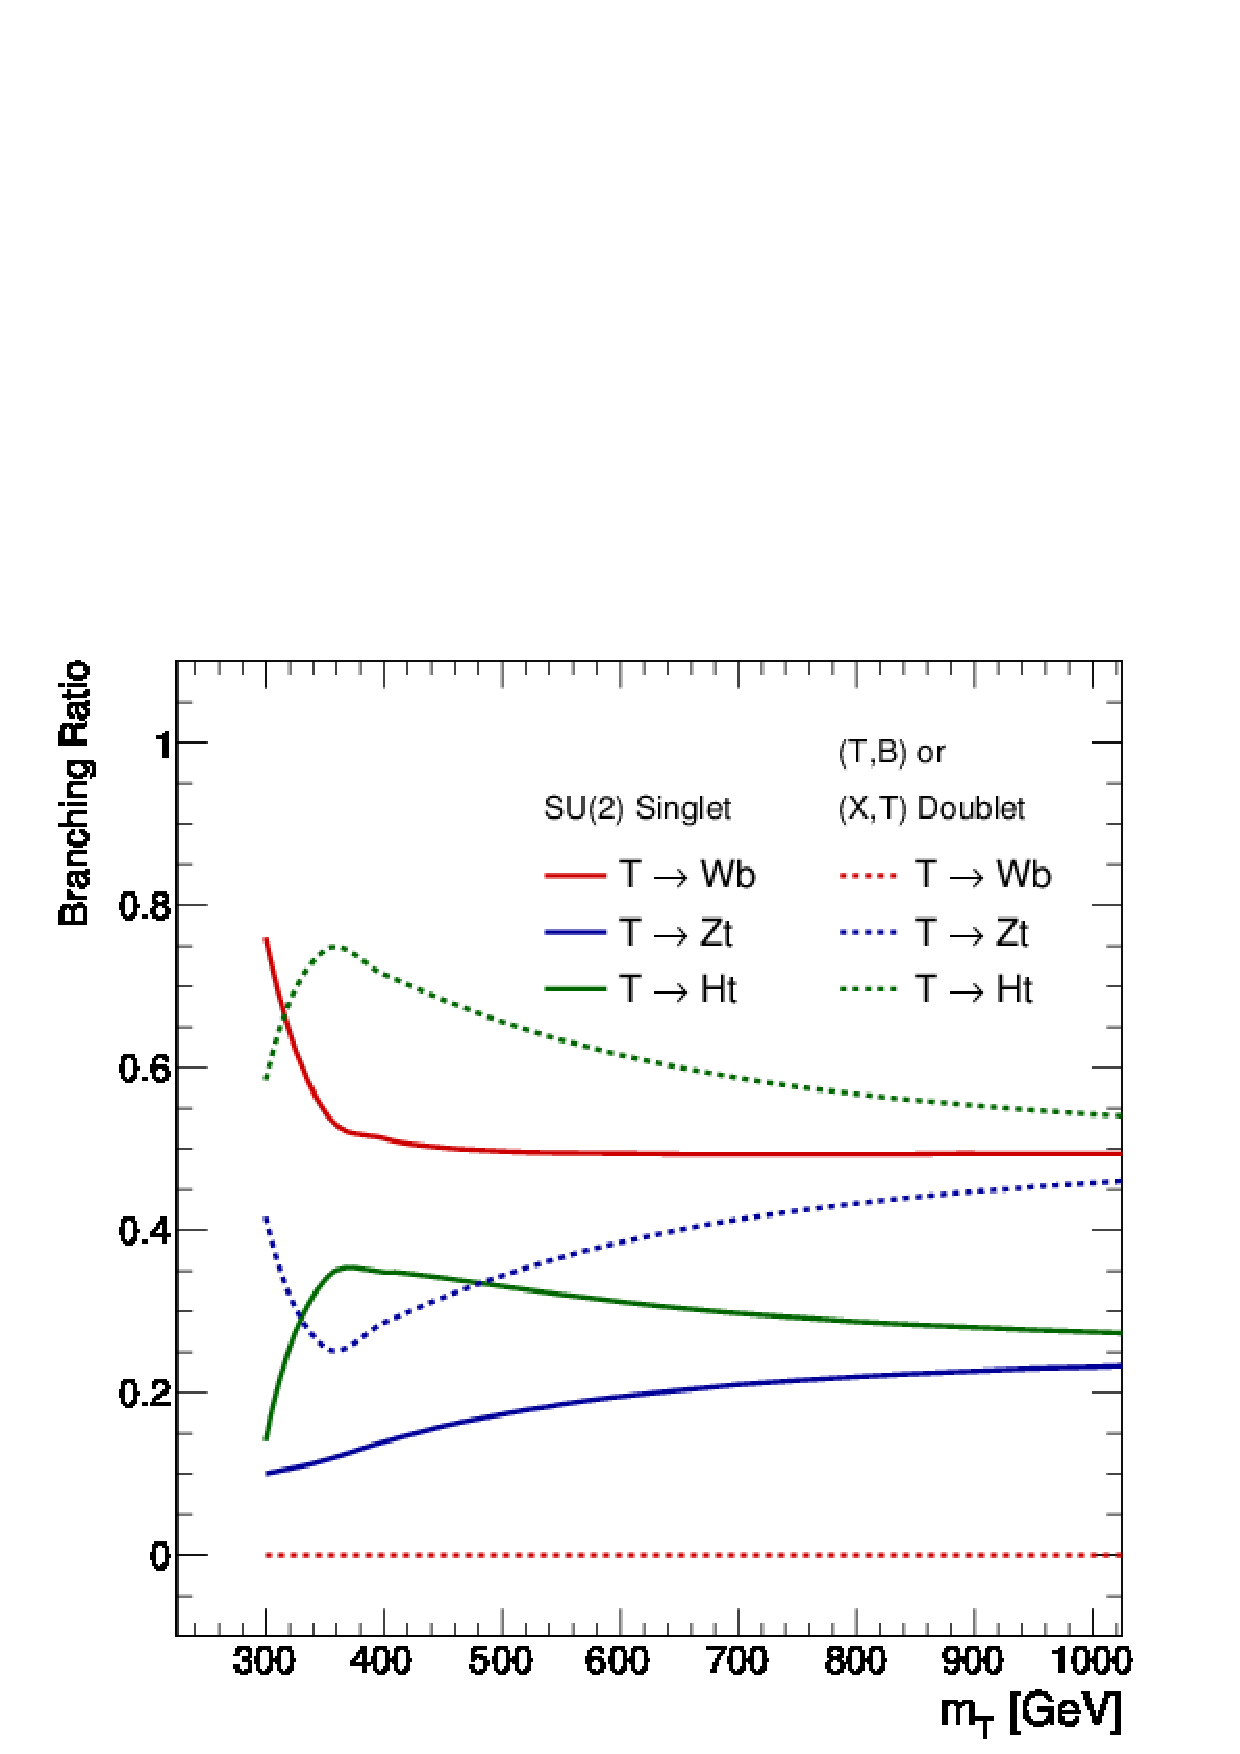
\includegraphics[width=0.95\textwidth]{../vlq_analysis/figures/fig_02a.pdf}
\end{minipage}

\end{frame}




\begin{frame}\frametitle{Model Independent Strategy}
\footnotesize\centering


\begin{pgfpicture}{0.0\textwidth}{0.0\textheight}{1.\textwidth}{.6\textwidth}

\begin{pgfscope}
\pgfdeclareimage[interpolate=true,width=.45\textwidth]{tab}{pics/tabBRs}
\onslide<1->{
    \pgfsetendarrow{\pgfarrowlargepointed{6pt}}
    \pgfsetlinewidth{1.5pt}
    \usebeamercolor[fg]{head/foot boxes}
    \begin{pgftranslate}{\pgfpoint{0.07\textwidth}{0.15\textheight}}
\pgfline{\pgfxy(0,0)}{\pgfxy(5.5,0)}
\pgfstroke
\pgfputat{\pgfxy(3.5,-0.5)}{\pgfbox[left,base]{BR($T\to Wb$)}}
    \usebeamercolor[fg]{normal text}
\pgfcircle[fill]{\pgfxy(6.8,4.1)}{2pt}
\pgfputat{\pgfxy(7,4)}{\pgfbox[left,base]{Build a 2-dim plane}}
\pgfputat{\pgfxy(7,3.7)}{\pgfbox[left,base]{to scan model mixing}}
%    \end{pgftranslate}
%\end{pgfscope}
}
%\pause
\onslide<2->{
%\begin{pgfscope}
    \pgfsetendarrow{\pgfarrowlargepointed{6pt}}
    \pgfsetlinewidth{1.5pt}
    \usebeamercolor[fg]{head/foot boxes}
%    \begin{pgftranslate}{\pgfpoint{0.1\textwidth}{0.15\textheight}}
    \usebeamercolor[fg]{head/foot boxes}
\pgfline{\pgfxy(0,0)}{\pgfxy(0,5.5)}
\pgfstroke
    \begin{pgfrotateby}{\pgfdegree{90}}
\pgfputat{\pgfxy(3.5,0.4)}{\pgfbox[left,base]{BR($T\to Ht$)}}
    \end{pgfrotateby}
%    \end{pgftranslate}
%\end{pgfscope}
    \usebeamercolor[bg]{head/foot boxes}
    \pgfcircle[fill]{\pgfxy(5.,0)}{3pt}
    \pgfcircle[fill]{\pgfxy(2.5,1.5)}{3pt}
    \pgfcircle[fill]{\pgfxy(0.,3.)}{3pt}
    \pgfputat{\pgfxy(5.5,4.7)}{\pgfbox[left,base]{\pgfuseimage{tab}}}
}
%\pause
\onslide<3->{
%\begin{pgfscope}
    \pgfsetlinewidth{1.5pt}
    \color{light-gray}
%    \begin{pgftranslate}{\pgfpoint{0.1\textwidth}{0.15\textheight}}
%\pgfline{\pgfxy(5,0)}{\pgfxy(0,5)}
%\pgfstroke
\pgfmoveto{\pgfxy(5,0)}
\pgflineto{\pgfxy(5,5)}
\pgflineto{\pgfxy(0,5)}
%\pgfstroke
\pgffill
    \color{gray}
\pgfputlabelrotated{0.5}{\pgfxy(0,5)}{\pgfxy(5,0)}{8pt}{\pgfbox[center,base]{Forbidden}}
    \usebeamercolor[fg]{normal text}
\pgfcircle[fill]{\pgfxy(6.8,3.3)}{2pt}
\pgfputat{\pgfxy(7,3.2)}{\pgfbox[left,base]{Sum of BRs is 1$^{(a)}$}}
%\pgfputat{\pgfxy(5.2,0.7)}{\pgfbox[left,base]{\scriptsize $^{(a)}$BR($T\to  Zt/b$) = 1 - BR($T\to Ht/b$) - BR($T\to Wb/t$)}}
\pgfputat{\pgfxy(5.9,-0.9)}{\pgfbox[left,base]{\scriptsize $^{(a)}$BR($T\to  Zt$) = 1 - BR($T\to Ht$) - BR($T\to Wb$)}}
%\pgfputat{\pgfxy(8.755,-0.7)}{\pgfbox[left,base]{\scriptsize - BR($T\to Wb$)}}
{
    \usebeamercolor[bg]{head/foot boxes}
    \pgfcircle[fill]{\pgfxy(5.,0)}{3pt}
}
%    \end{pgftranslate}
%\end{pgfscope}
}
%\pause
\onslide<4->{
%\begin{pgfscope}
    \pgfsetlinewidth{1.5pt}
%    \begin{pgftranslate}{\pgfpoint{0.1\textwidth}{0.15\textheight}}
    \usebeamercolor[fg]{normal text}
\pgfcircle[fill]{\pgfxy(6.8,2.8)}{2pt}
\pgfputat{\pgfxy(7,2.7)}{\pgfbox[left,base]{Different analyses are}}
\pgfputat{\pgfxy(7,2.4)}{\pgfbox[left,base]{sensitive to different areas}}
    \usebeamercolor[fg]{head/foot boxes}
\begin{pgfscope}
\pgfmoveto{\pgfxy(5,0)}
\pgflineto{\pgfxy(0,0)}
\pgflineto{\pgfxy(0,5)}
\pgfclip
\pgfcircle[fill]{\pgfxy(.5,4)}{55pt}
{\usebeamercolor[bg]{normal text}
%\pgfputat{\pgfxy(0.,3.5)}{\begin{pgfrotateby}{\pgfdegree{-45}}\pgfbox[left,base]{$T(B)\to Ht(b)$}\end{pgfrotateby}}
\pgfputat{\pgfxy(0.05,3.2)}{\pgfbox[left,base]{\large$Ht+X$}}
}
{
    \usebeamercolor[bg]{head/foot boxes}
    \pgfcircle[fill]{\pgfxy(0.,3.)}{3pt}
}
}
\pgfcircle[fill]{\pgfxy(4,0)}{35pt}
{\usebeamercolor[bg]{normal text}
%\pgfputat{\pgfxy(3.,0.4)}{\pgfbox[left,base]{$T(B)\to Wb(t)$}}
\pgfputat{\pgfxy(2.9,0.2)}{\pgfbox[left,base]{\large$Wb+X$}}
}
{
    \usebeamercolor[bg]{head/foot boxes}
    \pgfcircle[fill]{\pgfxy(5.,0)}{3pt}
}
\end{pgfscope}
\onslide<5->{
\usebeamercolor[fg]{normal text}
%\pgfcircle[fill]{\pgfxy(6.8,2.)}{2pt}
%\pgfputat{\pgfxy(7,1.9)}{\pgfbox[left,base]{Set exclusion using $CL_{s}$ }}
%\pgfputat{\pgfxy(7,1.6)}{\pgfbox[left,base]{in each point of the plane}}
%\pgfcircle[fill]{\pgfxy(6.8,1.2)}{2pt}
\pgfputat{\pgfxy(5.3,1.)}{\pgfbox[left,base]{\begin{tabular}{c c c} 
Set strategy & \multirow{2}{*}{$\Rightarrow$} & Check good bkg \\
($S/B$)      &                                & modeling \\
             &                                &  $\Downarrow$\\
Test \cls{b} and & \multirow{2}{*}{$\Leftarrow$} & \multirow{2}{*}{Look at data} \\
\cls{s+b} hypotheses & &\\
\multicolumn{3}{c}{$\nwarrow$} \\
\multicolumn{3}{c}{\it for each point of the BR plane}\\
\end{tabular}}}
}
    \end{pgftranslate}
\end{pgfscope}
\end{pgfpicture}

\end{frame}





\begin{frame}\frametitle{Preselection}
\centering\myskip

\begin{minipage}{.6\textwidth}\centering\footnotesize
Two searches using common analysis framework:
\begin{minipage}{.5\textwidth}\centering
\begin{itemize}
\item \wbx
\end{itemize}
\scriptsize
\cccolor 

ATLAS-CONF-2013-060~\cite{ATLAS-CONF-2013-060}
\end{minipage}\begin{minipage}{.5\textwidth}\centering
\begin{itemize}
\item \htx
\end{itemize}
\scriptsize
\cccolor 

ATLAS-CONF-2013-018~\cite{ATLAS-CONF-2013-018}
\end{minipage}

\myskip

\begin{tabular}{ll}
\toprule
Preselection stage & Requirements \\
\midrule
Single lepton & One electron or muon\\
              & matching trigger  \\\midrule
%\\
QCD rejection & $\met >20\gev$\\
              & $\met +m_{\rm T}>60\gev$ \\\midrule
%\\
Jet multiplicity & $\geq 4$ jets\\
                 & $\geq 1$ $b$-tagged jets \\
\bottomrule\end{tabular}

\myskip
{\bfseries\cccolor + ``orthogonality'' requirements} 

\myskip

\end{minipage}\begin{minipage}{.4\textwidth}\centering
\vskip-5ex
\includegraphics[width=0.9\textwidth]{pics/feyn_wbwb}\\
\vskip-2ex
\includegraphics[width=0.9\textwidth]{pics/feyn_htX}
\end{minipage}


\end{frame}



\begin{frame}\frametitle{Background and signal modelling}
\centering\myskip

\begin{minipage}{.5\textwidth}\footnotesize\centering
\scriptsize
Yields in the preselection region ``blinded'' as:\\
$\htfj<800\gev$ (*)
\myskip

  \input{tabs/blinded_presel}

\myskip
(*) $\htfj = \pT(l) + \met + \sum_{j = 1}^{\rm 4}\pT(j)$

\begin{pgfpicture}{0.0\textwidth}{0.0\textheight}{1.\textwidth}{.01\textwidth}
\pgfdeclareimage[interpolate=true,width=0.8\textwidth]{ttalp}{pics/Njets25_ELEMUON_4jetin1btagin_NOMINAL}
\begin{pgfscope}
 \pgfsetlinewidth{1.pt}
 \usebeamercolor[bg]{head/foot boxes}
 \pgfrect[stroke]{\pgfxy(0,4.15)}{\pgfxy(6,0.35)}
\only<2>{
\pgfputat{\pgfxy(0.8,0.2)}{\pgfbox[left,base]{\pgfuseimage{ttalp}}}
}
\end{pgfscope}
\end{pgfpicture}

\end{minipage}\begin{minipage}{.5\textwidth}\footnotesize\centering

\only<1>{
\begin{itemize}
\item $t\bar{t}$ pair production in association with jets generated with {\tt MC@NLO}+{\tt HERWIG}
\item $m_t = 172.5\gev$
\item NNLO theoretical cross section
\end{itemize}

but\\
{\tt MC@NLO} does not model well high-jet multiplicity regions!

}

\only<2>{
\begin{itemize}
\item Additional samples generated with {\tt ALPGEN}+{\tt HERWIG}
\item Separate samples are generated for $t\bar{t}$+light jets with up to three additional light partons,
and for $t\bar{t}$+heavy-flavour jets including $t\bar{t}b\bar{b}$ and $t\bar{t}c\bar{c}$ 
\item $m_t = 172.5\gev$
\item NNLO theoretical cross section
\end{itemize}

Yields for \ttbar\ predicted with \texttt{ALPGEN}
are $\sim$3-8\% higher than \texttt{MC@NLO}

%\includegraphics[width=0.8\textwidth]{pics/Njets25_ELEMUON_4jetin1btagin_NOMINAL}

}

\end{minipage}

\end{frame}


\begin{frame}\frametitle{Background and signal modelling}
\centering\myskip

\begin{minipage}{.5\textwidth}\footnotesize\centering
\scriptsize
Yields in the preselection region ``blinded'' as:\\
$\htfj<800\gev$ (*)
\myskip

  \input{tabs/blinded_presel}

\myskip
(*) $\htfj = \pT(l) + \met + \sum_{j = 1}^{\rm 4}\pT(j)$

\begin{pgfpicture}{0.0\textwidth}{0.0\textheight}{1.\textwidth}{.01\textwidth}
\begin{pgfscope}
 \pgfsetlinewidth{1.pt}
 \usebeamercolor[bg]{head/foot boxes}
 \pgfrect[stroke]{\pgfxy(0,3.5)}{\pgfxy(6,0.7)}
\end{pgfscope}
\end{pgfpicture}

\end{minipage}\begin{minipage}{.5\textwidth}\footnotesize\centering


\begin{itemize}
\item $W$ and $Z$ boson production in association with jets generated with up to five additional partons with {\tt ALPGEN}+{\tt HERWIG}
\end{itemize}

$W$+jets:
\begin{itemize}
\item Samples generated separately for $W$+light jets, $Wb\bar{b}$+jets, $Wc\bar{c}$+jets, and $Wc$+jets
\item Normalized to data-driven prediction
\end{itemize}

$Z$+jets:
\begin{itemize}
\item Samples generated separately for $Z$+light jets, $Zb\bar{b}$+jets, and $Zc\bar{c}$+jets 
\item Inclusive NNLO theoretical cross section
\end{itemize}

\end{minipage}
\end{frame}




\begin{frame}\frametitle{Background and signal modelling}
\centering\myskip

\begin{minipage}{.5\textwidth}\centering
\scriptsize
Yields in the preselection region ``blinded'' as:\\
$\htfj<800\gev$ (*)
\myskip

  \input{tabs/blinded_presel}

\myskip
(*) $\htfj = \pT(l) + \met + \sum_{j = 1}^{\rm 4}\pT(j)$


\begin{pgfpicture}{0.0\textwidth}{0.0\textheight}{1.\textwidth}{.01\textwidth}
\begin{pgfscope}
 \pgfsetlinewidth{1.pt}
 \usebeamercolor[bg]{head/foot boxes}
 \pgfrect[stroke]{\pgfxy(0,3.27)}{\pgfxy(6,0.35)}
\end{pgfscope}
\end{pgfpicture}

\end{minipage}\begin{minipage}{.5\textwidth}\footnotesize
\centering

\begin{itemize}
\item QCD multi-jet events have high cross-section
\item Jets are misidentified as leptons
\item Data-driven estimation (Matrix-method)
\end{itemize}

\includegraphics[width=0.4\textwidth]{../vlq_analysis/figures/mm_regions}

\myskip

\begin{minipage}{.7\textwidth}\footnotesize
$N^\mathrm{loose}  =  N^\mathrm{loose}_\mathrm{real} + N^{loose}_\mathrm{fake}$ \\\myskip
$N^\mathrm{tight}  =  \epsilon_\mathrm{real}N^\mathrm{loose}_\mathrm{real} + \epsilon_\mathrm{fake}N^\mathrm{loose}_\mathrm{fake}$
\end{minipage}

%N^\mathrm{tight}_\mathrm{fake} = \frac{\epsilon_\mathrm{fake}}{\epsilon_\mathrm{real} - \epsilon_\mathrm{fake}}(N^\mathrm{loose} \epsilon_\mathrm{real} - N^\mathrm{tight})$$

\end{minipage}
\end{frame}


\begin{frame}\frametitle{Background and signal modelling}
\centering\myskip

\begin{minipage}{.5\textwidth}\footnotesize\centering
\scriptsize
Yields in the preselection region ``blinded'' as:\\
$\htfj<800\gev$ (*)
\myskip

  \input{tabs/blinded_presel}

\myskip
(*) $\htfj = \pT(l) + \met + \sum_{j = 1}^{\rm 4}\pT(j)$

\begin{pgfpicture}{0.0\textwidth}{0.0\textheight}{1.\textwidth}{.01\textwidth}
\begin{pgfscope}
 \pgfsetlinewidth{1.pt}
 \usebeamercolor[bg]{head/foot boxes}
 \pgfrect[stroke]{\pgfxy(0,2.7)}{\pgfxy(6,0.6)}
\end{pgfscope}
\end{pgfpicture}

\end{minipage}\begin{minipage}{.5\textwidth}\footnotesize\centering

Single top:
\begin{itemize}
\item $s$-channel and $Wt$ production generated with {\tt MC@NLO}+{\tt HERWIG}
\item $t$-channel generated with {\tt ACERMC}+{\tt PYTHIA}
\item $m_t = 172.5\gev$
\item NNLO theoretical cross sections
\end{itemize}

Diboson:

\begin{itemize}
\item Diboson production generated with {\tt HERWIG}
\item NLO theoretical cross section
\end{itemize}

\end{minipage}
\end{frame}



\begin{frame}\frametitle{Background and signal modelling}
\centering\myskip

\begin{minipage}{.5\textwidth}\footnotesize\centering
\scriptsize
Yields in the preselection region ``blinded'' as:\\
$\htfj<800\gev$ (*)
\myskip

  \input{tabs/blinded_presel}

\myskip
(*) $\htfj = \pT(l) + \met + \sum_{j = 1}^{\rm 4}\pT(j)$

\begin{pgfpicture}{0.0\textwidth}{0.0\textheight}{1.\textwidth}{.01\textwidth}
\begin{pgfscope}
 \pgfsetlinewidth{1.pt}
 \usebeamercolor[bg]{head/foot boxes}
 \pgfrect[stroke]{\pgfxy(0,2.15)}{\pgfxy(6,0.6)}
\end{pgfscope}
\end{pgfpicture}

\end{minipage}\begin{minipage}{.5\textwidth}\footnotesize\centering

$t\bar{t}V$:
\begin{itemize}
\item $t\bar{t}$ produced in association with a $W$ or $Z$ boson generated with {\tt MADGRAPH}+{\tt PYTHIA}
\item $m_t = 172.5\gev$
\item NLO theoretical cross section
\end{itemize}

$t\bar{t}H$:
\begin{itemize}
\item $t\bar{t}$ produced in association with a Higgs boson generated with {\tt PYTHIA}
\item $m_t = 172.5\gev$, $m_H=125\gev$
\item Higgs decay modes considered: $H\to b\bar{b}$, $c\bar{c}$, $gg$, $W^+W^-$
\item NLO theoretical cross section
\end{itemize}

\end{minipage}
\end{frame}



\begin{frame}\frametitle{Background and signal modelling}
\centering\myskip

\begin{minipage}{.5\textwidth}\footnotesize\centering
\scriptsize
Yields in the preselection region ``blinded'' as:\\
$\htfj<800\gev$ (*)
\myskip

  \input{tabs/blinded_presel}

\myskip
(*) $\htfj = \pT(l) + \met + \sum_{j = 1}^{\rm 4}\pT(j)$

\begin{pgfpicture}{0.0\textwidth}{0.0\textheight}{1.\textwidth}{.01\textwidth}
\begin{pgfscope}
 \pgfsetlinewidth{1.pt}
 \usebeamercolor[bg]{head/foot boxes}
 \pgfrect[stroke]{\pgfxy(0,1.2)}{\pgfxy(6,0.35)}
\end{pgfscope}
\end{pgfpicture}

\end{minipage}\begin{minipage}{.5\textwidth}\footnotesize\centering

\begin{itemize}
\item \TTbar\ singlet production generated with {\tt PROTOS}+{\tt PYTHIA}
\item Branching ratio to each decay mode  ($Wb$, $Zt$ and $Ht$) is set to  1/3
\item Events are reweighted at the analysis level in order to reproduce any desired branching ratio configuration
\item $m_{T}$ values generated from $350\gev$ to $850\gev$ in steps of $50\gev$
\item $m_H=125\gev$, all Higgs boson decay modes are considered
\item NNLO theoretical cross section
\end{itemize}

\end{minipage}


\end{frame}

\begin{frame}\frametitle{Systematic uncertainties - Shape and Norm}
\centering\myskip\scriptsize

\resizebox{!}{.28\textwidth}{
\begin{tabular}{lcccc}
\toprule
Systematic uncertainty & \multicolumn{2}{c}{ \wbx\  } & \multicolumn{2}{c}{ \htx\  }\\
 & Status  & Components & Status  & Components\\
\midrule
Luminosity                  &  N & 1 &  N & 1\\
Lepton ID+reco+trigger      &  N & 1 &  N & 1\\
\rowcolor{TabLight}Jet energy scale            & SN & 1 & SN & 8\\
Jet energy resolution       & SN & 1 & SN & 1\\
%Jet mass scale               & - & -\\
%Jet mass resolution      & - & -\\
Jet vertex fraction efficiency & SN & 1 & SN & 1\\
\rowcolor{TabLight}$b$-tagging efficiency      & SN & 9 & SN & 9\\
$c$-tagging efficiency      & SN & 5 & SN & 5\\
Light jet-tagging efficiency    & SN & 1 & SN & 1\\\midrule
$t\bar{t}$ cross section    &  N & 1 &  N & 1\\
$t\bar{t}V$ cross section   &  N & 1 &  N & 1\\
$t\bar{t}H$ cross section   & - & - &  N & 1\\
Dibosons cross section      &  N & 1 &  N & 1\\
Single top cross section    &  N & 1 &  N & 1\\\midrule
$W$+jets normalization      &  N & 5 &  - & -\\
$Z$+jets normalization      &  N & 1 &  - & -\\
$V$+jets normalization      &  - & - &  N & 1\\
Multijet normalization      &  - & - &  N & 1\\
\rowcolor{TabLight}$t\bar{t}$ modelling        & SN & 3 & SN & 3\\
$V$+jets modelling         & SN & 1 &  - & -\\
$t\bar{t}$+heavy-flavour fractions &  - & -& N & 1\\
%$\TT$ modelling        & - & -\\
\bottomrule
\end{tabular}
}

\end{frame}



%----------------------------------
\section{Search for \TTbar\ decaying to $Wb+X$}
%----------------------------------

%----------------------------------
\section{Search for \TTbar\ decaying to $Ht+X$}
%----------------------------------

%----------------------------------
\section{Final results}
%----------------------------------

%----------------------------------
\section{Conclusions and outlook}
%----------------------------------


\appendix


\section*{References}
\setbeamertemplate{bibliography item}[text]

\begin{frame}[allowframebreaks]
\frametitle{References}\footnotesize
\bibliographystyle{unsrt}
%\bibliographystyle{myunsrt}
\bibliography{../bibliography/biblio}
\end{frame}


\section*{Backup}

%----------------------------------
\begin{frame}
 \frametitle{}

\begin{center}{\bfseries
BACKUP SLIDES}
\end{center}
\end{frame}


\begin{frame}\frametitle{LHC parameters}
\footnotesize\centering\myskip
\begin{table}\centering
	\begin{tabular}{lllll}\toprule
        Parameter                       & designed      &       2010 &  2011     &   2012\\ \midrule
        Beam energy (\tev/c)            & 7             & 3.5        & 3.5       & 4    \\
        Beta function $\beta*$ (m)      & 0.55          & 2.0/3.5    & 1.5/1.0   & 0.6  \\
        Max. No. bunches/beam           & 2808          & 368        & 1380      &1380  \\
        Max. No. protons/bunch          & 1.15$\times10^{11}$ & 1.2$\times10^{11}$ & 1.45$\times10^{11}$ & 1.7$\times10^{11}$ \\
        Bunch spacing (ns)              & 25            & 150       & 75/50        & 50 \\
        Peak luminosity (\cmm2\sm1)     & 1$\times10^{34}$& 2.1$\times10^{32}$& 3.7$\times10^{33}$& 7.7$\times10^{33}$\\
        Emittance $\varepsilon_{n}$ ($\mu$rad)&3.75     &   2.0      & 2.4      & 2.5   \\
        Max. $<\mu>$                    & 19            & 4             & 17         & 37       \\
	\bottomrule\end{tabular}\caption{Overview of some parameters for the LHC performance comparing the design values with their time
        evolution during the first long run operation in 2010-2013~\cite{Lamont}.}\label{tab:lhcpar}
\end{table}

\end{frame}



\end{document}
